\documentclass[pdftex,10pt]{article}
\usepackage{multicol}
\usepackage[ampersand]{easylist}
\usepackage{tikz}
\usepackage{tabularx}
\usepackage{float}
\usetikzlibrary{intersections}
\usetikzlibrary{decorations.pathreplacing}

\title{Hierarchy of Computer Architecture \\ Final Project, CIS-242-AA-CRN94413}
\author{Leigh Johnson \\ johnsonl6@my.smccd.edu \\ Cañada College}

\begin{document}
\maketitle

\tableofcontents

\section{Hierarchy of Computer Architecture}
\begin{figure}[h]
    \centering
    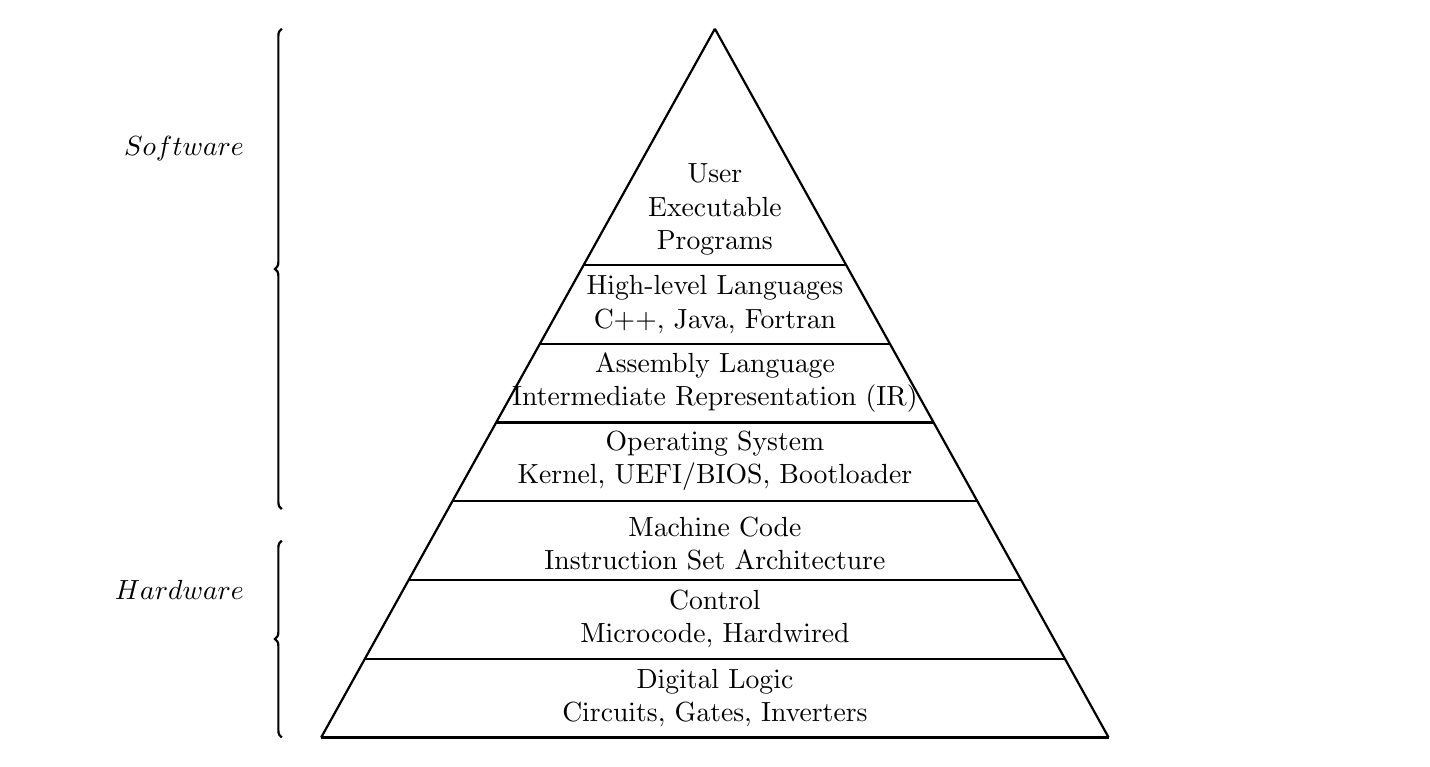
\begin{tikzpicture}[thick]

        \coordinate (A) at (-5,0) {};
        \coordinate (B) at ( 5,0) {};
        \coordinate (C) at (0,9) {};
        \draw[name path=AC] (A) -- (C);
        \draw[name path=BC] (B) -- (C);
        \foreach \y/\A in {
        0/{Digital Logic\\ Circuits, Gates, Inverters},
        1/{Control\\ Microcode, Hardwired},
        2/{Machine Code\\ Instruction Set Architecture},
        3/{Operating System\\Kernel, UEFI/BIOS, Bootloader},
        4/{Assembly Language\\Intermediate Representation (IR)},
        5/{High-level Languages\\C++, Java, Fortran},
        6/User\\Executable\\Programs} {
        \path[name path=horiz] (A|-0,\y) -- (B|-0,\y);
        \draw[name intersections={of=AC and horiz,by=P},
            name intersections={of=BC and horiz,by=Q}] (P) -- (Q)
        node[midway,above,align=center,text width=
            \dimexpr(7em-\y em)*7\relax] {\A};
        }

        \draw [decorate,
            decoration = {brace}] (-5.5,0) --  (-5.5,2.5)
        node[pos=0.75,left=10pt,black]{$Hardware$};
        \draw [decorate,
            decoration = {brace}] (-5.5,2.9) --  (-5.5,9)
        node[pos=0.75,left=10pt,black]{$Software$};
    \end{tikzpicture}
    \caption{\bf{Abstract Levels of a Computer System}}
\end{figure}

Computer architecture hierarchy refers to the structured organization of components within a computer system. This hierarchy typically starts with the smallest, simplest elements like transistors and builds up to more complex structures such as logic gates, microprocessors, and finally an entire computer operating system capable of running user programs. The components become more integrated and complex at each level of this hierarchy.

\section{Digital Logic}

The \textbf{Digital Logic} layer includes the physical components of the computer, like circuits, gates, and wires. Logic gates are the fundamental building block and implement operations using \textbf{Boolean Logic}.

\subsection{Boolean Algebra}

Named after mathematician George Boole, Boolean laws and identities can be used to reduce/simplify a logical statement. In the context of computer science, simpler circuits are preferred because they consume fewer resources (energy, money) and are simpler to build.

\begin{table}[htbp]
    \abovedisplayskip=-5pt
    \belowdisplayskip=-5pt
    \centering
    \begin{tabularx}{\textwidth}{| X | X | X |}
        \hline
        Name                 & AND form              & OR form               \\ \hline
        \[Identity\]         & \[1x = 1\]            & \[0+x = x\]           \\ \hline
        \[Null\]             & \[0x = 0\]            & \[1 +x =1\]           \\ \hline
        \[Idempotent\]       & \[xx = x\]            & \[x + x = x\]         \\ \hline
        \[Inverse\]          & \[xx' = 0\]           & \[x + x' = 1\]        \\ \hline
        \[Null\]             & \[0x = 0\]            & \[1 +x =1\]           \\ \hline
        \[Commutative\]      & \[xy = yx\]           & \[x+y = y + x\]       \\ \hline
        \[Associative\]      & \[(xy)z = x(yz)\]     & \[(x+y)+z = x+(y+z)\] \\ \hline
        \[Distributive\]     & \[x+yz = (x+y)(x+z)\] & \[x(y+z) = xy+xz\]    \\ \hline
        \[Absorption\]       & \[x(x+y) = x\]        & \[x + xy = x\]        \\ \hline
        \[DeMorgan's\]       & \[(xy)' = x'+y'\]     & \[(x+y)' = x'y'\]     \\ \hline
        \[DoubleComplement\] & \[(x)'' = x\]         & \[(x)'' = x\]         \\ \hline
    \end{tabularx}
    \caption{Boolean Algebra Identities and Laws}

\end{table}

\subsection{Truth Tables}

Also known as \textbf{Karnaugh Maps (K-Maps)}, a \textbf{Truth Table} can be represented in two formats:
\begin{itemize}
    \item \textbf{Sum-of-Products form} - collection of ANDed variables (product terms) that are ORed together (sum of all product terms)
    \item \textbf{Product-of-Sums form} - collection of ORed variables (sum terms) that are ANDed together (product all summed terms)
\end{itemize}


Consider the following example of a function \textit{F(x,y,z) = x'yz + xy'z + xyz}, which outputs true (1) if the majority of inputs are true:

\begin{table}[htbp]
    \abovedisplayskip=-5pt
    \belowdisplayskip=-5pt
    \centering
    \begin{tabularx}{\textwidth}{| X | X | X | X |}
        \hline
        x & y & z & F(x,y,z) \\ \hline
        0 & 0 & 0 & 0        \\ \hline
        0 & 0 & 1 & 0        \\ \hline
        0 & 1 & 0 & 0        \\ \hline
        1 & 0 & 0 & 0        \\ \hline
        1 & 0 & 1 & 1        \\ \hline
        1 & 1 & 0 & 1        \\ \hline
        1 & 1 & 1 & 1        \\ \hline
    \end{tabularx}
    \caption{Truth Table representation for a majority function:\\ \textit{F(x,y,z) = x'yz + xy'z + xyz}.}

\end{table}


\subsection{Logic Gates}

Using \textbf{Boolean Algebra}, we can construct the next basic building block of digital circuitry: a \textbf{Logic Gate}. The most basic logic gates are:
\begin{itemize}
    \item \textbf{AND Gate} - true (1) if both inputs are true, otherwise false (0).
    \item \textbf{OR Gate} - true (1) if either input is true, false (0) if both inputs are false.
    \item \textbf{NOT Gate} - true (1) if the input is false (0), false if the input is true. Also known as an \textbf{Inverter}
\end{itemize}

Two other gates, \textbf{NAND} and \textbf{NOR}, produce complementary output to AND and OR gates. The NAND gate is called a \textbf{universal gate} because any electronic circuit can be constructed using only NAND gates.

\section{Hardware Control}

\textbf{Logic Gates} are combined to build different types of circuitry and modules. The simplest units are \textbf{Integrated Circuits (ICs)}, a chip consisting of the necessary transistors, resistors, and capacitors to implement various gates.

\subsection{Hardwired Control}
\subsubsection{Combinational Circuit}

\textbf{Combinational Circuits} use a stateless circuit design, which accepts input values and (almost) instantly produces an output. One of the simplest examples is the \textbf{Half Adder}, which outputs the sum of two bits.

\subsubsection{Sequential Circuit}

The output of \textbf{Seqential Circuits} varies depending on the internal state (memory) of the circuit. The state changes are governed by a \textbf{Clock}, which produces a regular periodic electrical wave. Sequential circuits typically incorporate a \textbf{Feedback Loop}, which loops output back to input terminals.

A \textbf{Finite State Machine (FSM)} depicts the relationship between the state of \textbf{Flip-Flop circuity} and the system clock. FSMs can only be in one state at a time.

\subsection{Microcode}

\textbf{Microcode} is a characteristic of \textbf{Complex Instruction Set Computers (CISC)}, which are a layer of low-level instructions needed by higher-level machine code instructions. Machine code is an intermediary between the machine language and the hardware, allowing more flexible control of the processor's operations. A \textbf{Microprogram} is a sequence of microcode instructions.

\subsection{Hardware Components of a Computer}


\subsubsection{Central Processing Unit (CPU)}

The \textbf{Central Processing Unit (CPU)} is responsible for fetching program instructions, decoding each instruction, and executing the decoded operations. These steps are known as the \textbf{Fetch-Decode-Execute Cycle} or \textbf{Instruction Cycle}.

\subsubsection{Memory}

Memory refers to the devices that store data temporarily or permanently.

\begin{itemize}
    \item \textbf{Random Access Memory (RAM)} - a volatile (temporary) form of memory.
    \item \textbf{Read-Only Memory (ROM)} - a nonvolatile (permanent) form of memory that is read-only.
    \item \textbf{Flash Memory (NAND, NOR)} - a non-volatile (permanent) form of memory that can be erased and rewritten.
\end{itemize}

\subsubsection{Storage}

A storage device is used to store data. There are many different kinds of storage mediums available for computers:

\begin{itemize}
    \item \textbf{Magnetic Tape} - a thin strip of plastic coated with a magnetizable material.
    \item \textbf{Optical Disks} - reflective disk read using a laser.
    \item \textbf{Hard Disk Drives (HDD)} - rotating "platter" disk with a magnetic head and seek arm.
    \item \textbf{Solid-State Drives (SSD)} - non-volatile flash memory.
\end{itemize}

\subsubsection{Bus (Communication)}

\subsubsection{MARIE Reference Architecture}
The CPU in the MARIE reference architecture (an example of \textbf{Von Neumann architecture}) consists of the following components:

\begin{itemize}
    \item \textbf{Arithmetic Logic Unit (ALU)} - performs logic operations (e.g., less-than or equals comparisons) and arithmetic (add, subtract).
    \item \textbf{Accumulator (AC)} - a specialized register used for storing the output of the last executed operation.
    \item \textbf{Input / Output Registers} - specialized registers used to store user input and program output.
    \item \textbf{Memory Buffer Register (MBR)} - specialized register used to store data being transferred to/from main memory.
    \item \textbf{Memory Address Register (MAR)} - specialized register used to store the memory address of data to be fetched from main memory.
    \item \textbf{Control Unit (CU)} - responsible for sequencing operations, manipulating the \textbf{Program Counter}.
    \item \textbf{Program Counter (PC)} - specialized register used to keep track of the next instruction to be executed.
    \item \textbf{Instruction Register (IR)} - specialized register used to hold the instruction currently being decoded/executed.
    \item \textbf{Main Memory} - also known as the datapath. Stores program data.
\end{itemize}


\section{Machine Code}

Machine code is the lowest-level computer language, consisting of binary or hexadecimal instructions.

\subsection{Instruction Set Architecture (ISA)}

An Instruction Set Architecture (ISA) is an agreed-upon interface between \textit{software} running on a machine and the \textit{hardware} that executes it.

The ISA provides the specification for:

\begin{itemize}
    \item Word size (e.g., 32-bit or 64-bit)
    \item Instruction opcodes and max operands
    \item Instruction length
    \item Addressing modes (e.g., byte-addressable or word-addressable)
    \item Supported data types and operations (e.g., IEEE 754 floating point arithmetic)
    \item Endianness (e.g. Big Endian or Little Endian)
    \item Branch evaluation
    \item Instruction Format
\end{itemize}

\subsection{Instruction Formats}

\begin{itemize}
    \item \textbf{Stack Architecture} - instructions and operands are popped off the stack. A stack architecture uses \textbf{postfix notation} (also known as Polish notation) to express operations.
    \item \textbf{Accumulator Architecture} - one operand of a binary operation is stored in the accumulator, one in memory.
    \item \textbf{General Purpose Register (GPR) Architecture} - operands stored in general-purpose registers.
\end{itemize}

\subsection{Reduced Instruction Set Architecture (RISC) vs. Complex Instruction Set Architecture (CISC)}
\begin{table}[H]
    \centering
    \begin{tabularx}{\textwidth}{| X | X |}
        \hline
        \textbf{RISC}                                       & \textbf{CISC}                                          \\ \hline
        Multiple register sets                              & Single register sets                                   \\ \hline
        Many registers (256+)                               & Few registers (6-16)                                   \\ \hline
        Parameter passing via on-chip register windows      & Parameter passing via off-chip memory (less efficient) \\ \hline
        Single-cycle instructions                           & Multi-cycle instructions                               \\ \hline
        Hardwired control                                   & Microcode Control                                      \\ \hline
        Highly pipelined                                    & Less Pipelined                                         \\ \hline
        Few Simple instructions                             & Many Complex instructions                              \\ \hline
        Fixed-length instructions                           & Variable-length instructions                           \\ \hline
        Complexity in compiler                              & Complexity in microcode                                \\ \hline
        Memory access is limited to load/store instructions & Many instructions can access memory                    \\ \hline
    \end{tabularx}
    \caption{Comparison of RISC and CISC attributes.}
\end{table}

\section{Operating System}

An operating system (OS) is the intermediary system software between users and the computer hardware. The OS facilitates the execution of application programs and efficiently manages hardware resources like CPU, memory, and I/O systems.

Operating System code is often referred to as \textbf{the Kernel}, especially to delineate between applications that run in \textbf{Kernel Space} vs. \textbf{User Space}

\subsection{Boot Firmware}

The following firmware is used during the computer boot stage. This firmware is responsible for initializing and testing system hardware components and loading the Bootloader or operating system.

\subsubsection{BIOS}

Basic Input/Output System (BIOS) is a legacy firmware interface initially developed by IBM. The UEFI standard has replaced BIOS, however the term "BIOS" is often used to refer to boot firmware in a generic sense.

\subsubsection{UEFI}

The Unified Extensible Firmware Interface (UEFI) is a specification that defines a software interface between an operating system and platform firmware, replacing the legacy Basic Input/Output System (BIOS) firmware interface. UEFI provides graphical menus, secure boot, and network capabilities before loading an operating system.

\section{Assembly Language}

Assembly is a human-readable language that compiles to \textbf{Machine Code}. Higher-order programming languages in the next section are compiled into Assembly Code or an \textbf{Intermediate Representation (IR)}.

\textbf{Intermediate Representations (IRs)} is an internal stage used by a compiler (e.g., LLVM) or virtual machine (e.g., Java Virtual Machine), which allows for optimizations and language/machine-agnostic conversion between source code and machine code.

\section{High-level Language}

A high-level language abstracts the implementation details of the machine, hardware, and instruction set. Examples of high-level languages include:

\begin{itemize}
    \item C/C++
    \item Rust
    \item Java
    \item Python
\end{itemize}

\section{User Space}

When a user writes and executes a program, this program typically runs in "user space" or "userland." This delineates between system applications that run in "kernel space" or "kernel land" and user programs.

\end{document}
